\section{Theory}

Our dataset consists of images.  One could use each individual pixel as an individual input feature, but that loses any relative spacial locality information between pixels, and is therefore prone to errors due to location in the image of the object to be identified \cite{lecun1998gradient}.  For example, if we want to identify if an image has a circle or not, looking at a set of pixels without knowing where they are located relative to eachother cannot be done in general.

For handwriting recognition, there are some features that some people have tried to extract to use in a learning algorithm.  These include aspect ratio, percent of thresholded pixels above the horizontal half plane, percent of thresholded pixels to the right of the vertical half plane, and so forth \cite{wikihandwritfeat}.  It is unknown if these features will be sufficient to classify the characters.

\subsection{Convolutional Neural Networks}

Early on in the project, we received a recommendation to use Convolutional Neural Networks (CNNs).  CNNs have been shown to be very effective in image recognition \cite{korekado2003convolutional} \cite{ciresan2012multi}.  One significant advantage of CNNs is the ability to make the representation \emph{invariant} to small translations of the input, such as for image recognition tasks \cite{Bengio-et-al-2015-Book}.  Another useful aspect of CNNs are their ability to automate feature identification and extraction \cite{Bengio-et-al-2015-Book}.

\begin{figure}[ht]
  \centering
  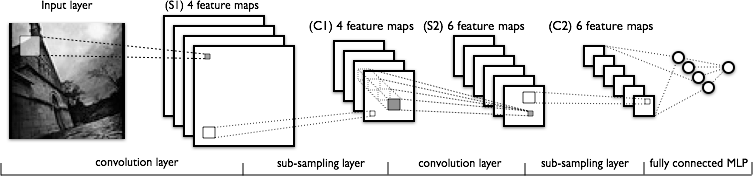
\includegraphics[width=\textwidth]{images/mylenet.png}
  \caption{
    Convolution and pooling layers that make up a CNN followed by a
    fully-connected Multi-layered Perceptron (MLP).
    (from \cite{Bengio-et-al-2015-Book})
    }
  \label{fig:convnet}
\end{figure}

CNNs are an example of multi-layered neural networks.

\subsection{Theano}

We were pointed by Dustin Webb to the Theano python module for implementation of CNNs.  Theano takes mathematical expressions and compiles them into C++ to make for a robust and efficient framework \cite{bergstra+al:2010-scipy}.  Theano was something completely new to us.  It uses symbolic expressions that can be compounded together.  You can define a loss function and have Theano symbolically generate the gradient for use in stochastic gradient descent.

\subsection{Linear Classifiers}

Even though we chose to use CNNs, we decided to first employ the linear classifiers we learned in class for comparison and to learn how to use Theano.  We chose to use Perceptron, Averaged Perceptron, SVM, and Logistic Regression.  These all can be implemented using stochastic gradient descent even though Perceptron is usually not directly implemented in that way.
